\clearpage

\section{Study of the effect of 12-sector (solar) oscillation parameters in the joint oscillation analysis}
\label{app:solar}

The effect of including solar parameters, $\sin^{2}2\theta_{12}$ and $\Delta m_{21}^{2}$, in the joint fit has been studied. These parameters 
were allowed to vary in the fit and were marginalized. As shown in Fig.~\ref{fig:solar}, confidence contours became larger when solar parameters 
are included in the fit. The best fit point for those parameters is at their extreme values allowed in the fit (see Fig.~\ref{fig:solarfit}), 
demonstrating that the joint analysis is unable to fit them, even for the estimated final POT. 


\begin{figure}[htbp]
\begin{center}
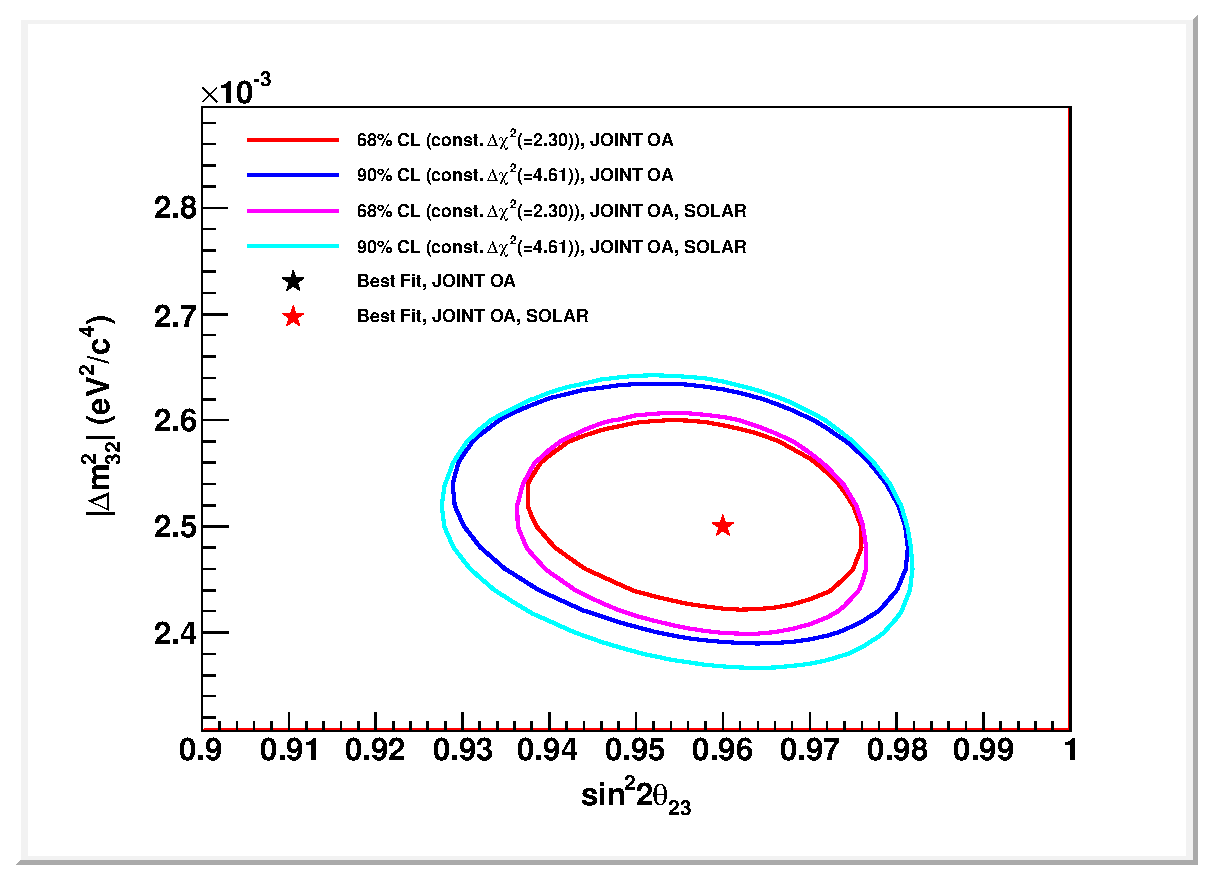
\includegraphics[width=0.7\textwidth]{images/validation/AppContoursJointOAMock100NewVsSolar.eps}
\caption{$\sin^{2}2\theta_{23}$ versus $\Delta m_{32}^{2}$ confidence regions for the estimated final POT (7$\times$10$^{21}$). 
Dark colors for the fit with fixed solar parameters and light colors for the fit with marginalized solar parameters. }
\label{fig:solar}
\end{center}
\end{figure}


\begin{figure}[htbp]
\begin{center}
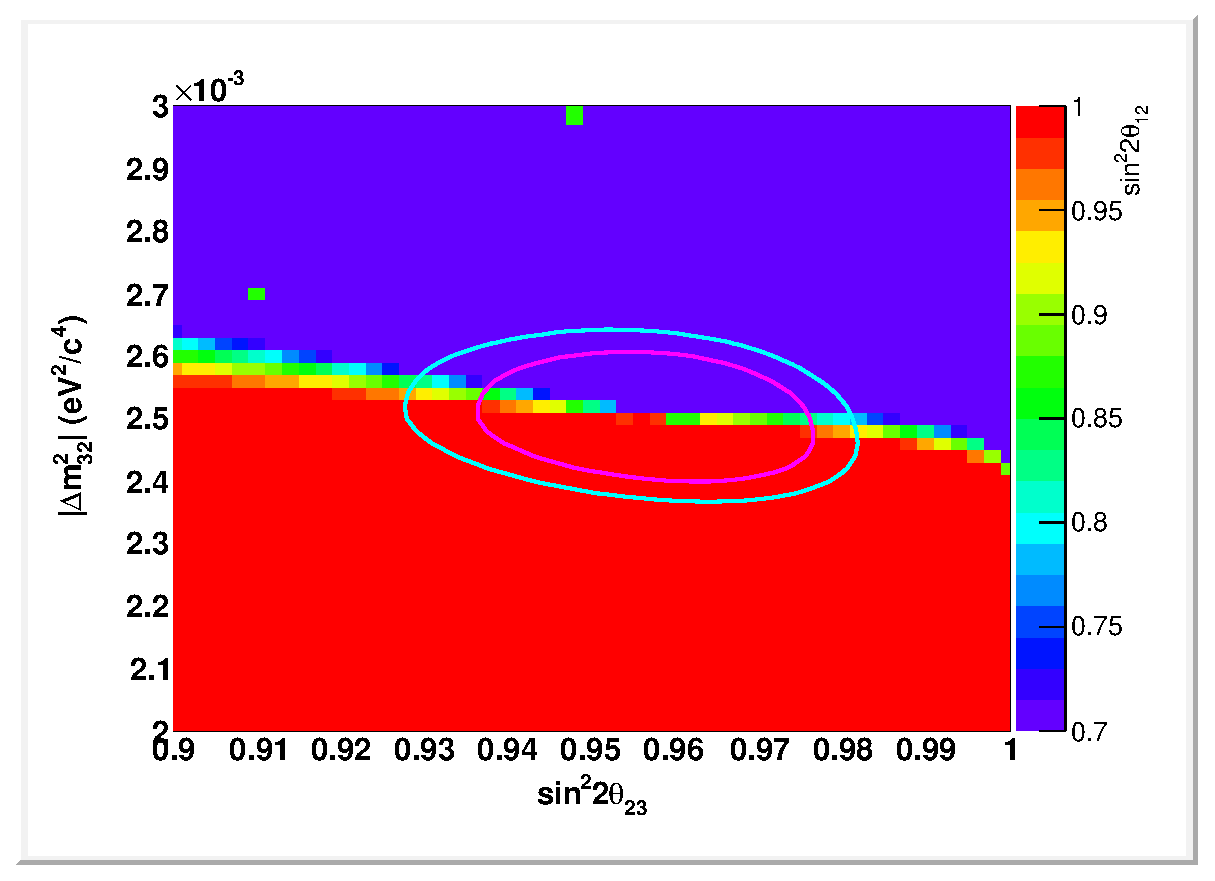
\includegraphics[width=0.49\textwidth]{images/validation/FittedTheta12JointFitSolar.eps}
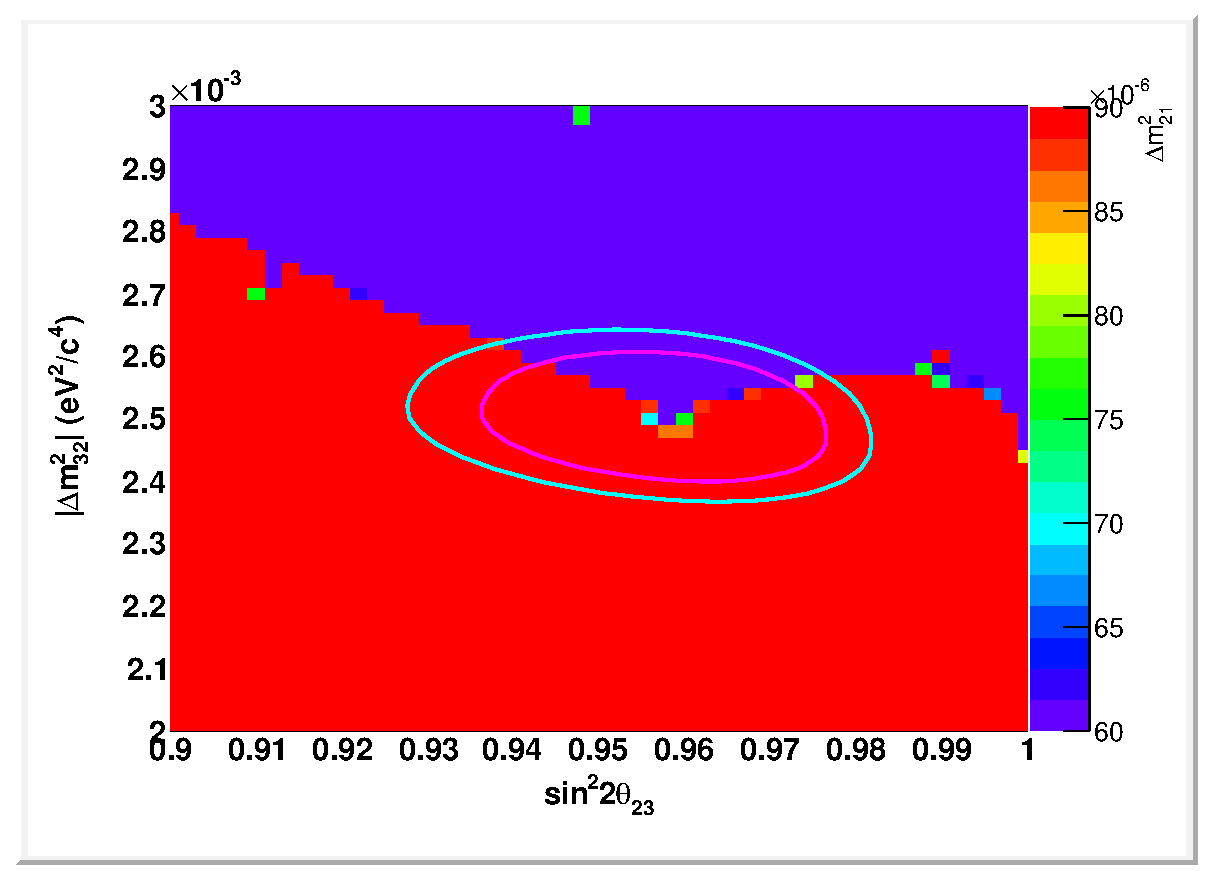
\includegraphics[width=0.49\textwidth]{images/validation/FittedDm12sqJointFitSolar.eps}
\caption{Fitted values of $\sin^{2}2\theta_{12}$ (left) and $\Delta m_{21}^{2}$ (right) for the joint fit with marginalized solar parameters, for the estimated final POT 
(7$\times$10$^{21}$).}
\label{fig:solarfit}
\end{center}
\end{figure}


